\documentclass[aspectratio=1610,slidestop,mathserif,final]{beamer}
\usepackage{Styles}
\def\footslide{Cours Freefem++ days 2016}

\begin{document}

\let\oldparskip=\parskip
\graphicspath{{./}{plots/}}
\ifpdf
\DeclareGraphicsExtensions{.pdf,.jpg,.tif,.gif}
\else
\DeclareGraphicsExtensions{.eps,.ps,.jpg,.gif}
\fi


\color{black}
%\section{Title Page}
% ======title page========================================================================
\setbeamertemplate{background}{
    \parbox[c][\paperheight]{\paperwidth}{
      \includegraphics[height=1.\paperheight,width=1.\paperwidth]{A_figs/jyulake.pdf}

    }}

\frame{

\begin{center}

{\Huge \bf\color{black}  FreeFem++ %, a tools to solving complex problem \\
%{\normalsize like Bose Einstein Condensate equation 
%or a  melting  problem.} 
}\\ ~\\
{\Huge
{\color{yellow} F. Hecht, O. Pironneau}}  \\

{\color{white} Laboratoire Jacques-Louis Lions} \\
{\color{white}   Universit\'e Pierre et Marie Curie \\ Paris,  France\\ ~}

\vfill \color{white} \normalsize 
with  {{\large I. Danaila, S. Auliac, P. Jolivet}}

\end{center}

\vfill \color{yellow}

 {\url{http://www.freefem.org} 
\hfill{\url{mailto:hecht@ann.jussieu.fr}}}

}
\setbeamertemplate{background}{}
\setbeamertemplate{footline}
{
\pgfputat{\pgfxy(2,0.5)}{\tiny \DarkGreen{\footslide} \hfil  \thepage/\pageref{LastPage} }
\pgfputat{\pgfxy(14.2,0.0)}{\logo}
%\rput[lt](3,0.29){\tiny \DarkGreen{ Modeling with finite elements, Minisymposium, U. Ljubljana, august 2011 } \hfill  \thepage }
%\rput[lt](11.2,0.5){\logo}
} 


%
%\newslide{movie} 
%\includemovie[repeat,autoplay, palindrome,mouse,rate=1]{20cm}{15cm}{/Users/hecht/work/Articles/MIT2/movies/ff.mp4}
%\end{frame}




\begin{frame} 
\manualFrameTitle{Outline}\scriptsize
\textBlack\tableofcontents\vfill\vfill\vfill\eject


\end{frame}

%%%AAA%%%




%\begin{frame} \manualFrameTitle{Outline} \textBlack\tableofcontents
%\end{frame}

\section{Introduction}

\newslide{Introduction} 
I suggest you choose, according to your level
\begin{itemize}
\item Beginners:  Follow the slides
\item Others 1: Follow today's example
\item Others 2: Suggest an example and receive help to program it.
\end{itemize}
Today's example:
\[
\rho\partial_t v - \frac1r\partial_r[\xi^f r\partial_r v+\xi^s r\partial_r d] =0,~~
\partial_t d = v,~r\in(R_0,R_1),~~v_{|R_0}=0,~v_{|R_1}=3,
\]
with $\rho=\rho^s{\bf 1}_{r\leq R} + \rho^f{\bf 1}_{r>R}$, $\xi^s=2c_1{\bf 1}_{r\leq R}$, $\xi^f= {\mu}{\bf 1}_{r>R}$, and with $d(r,0)=0$.
%
$$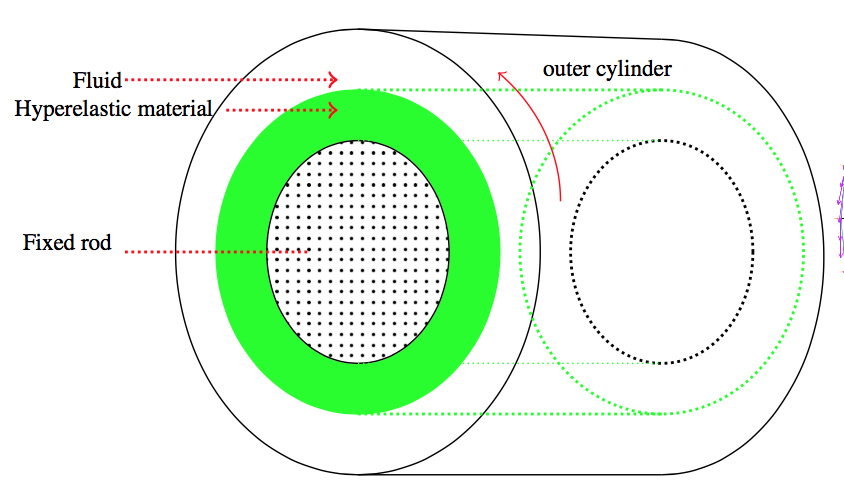
\includegraphics[width=6cm]{figure.png}$$
\end{frame}
%
\newslide{Example}
$$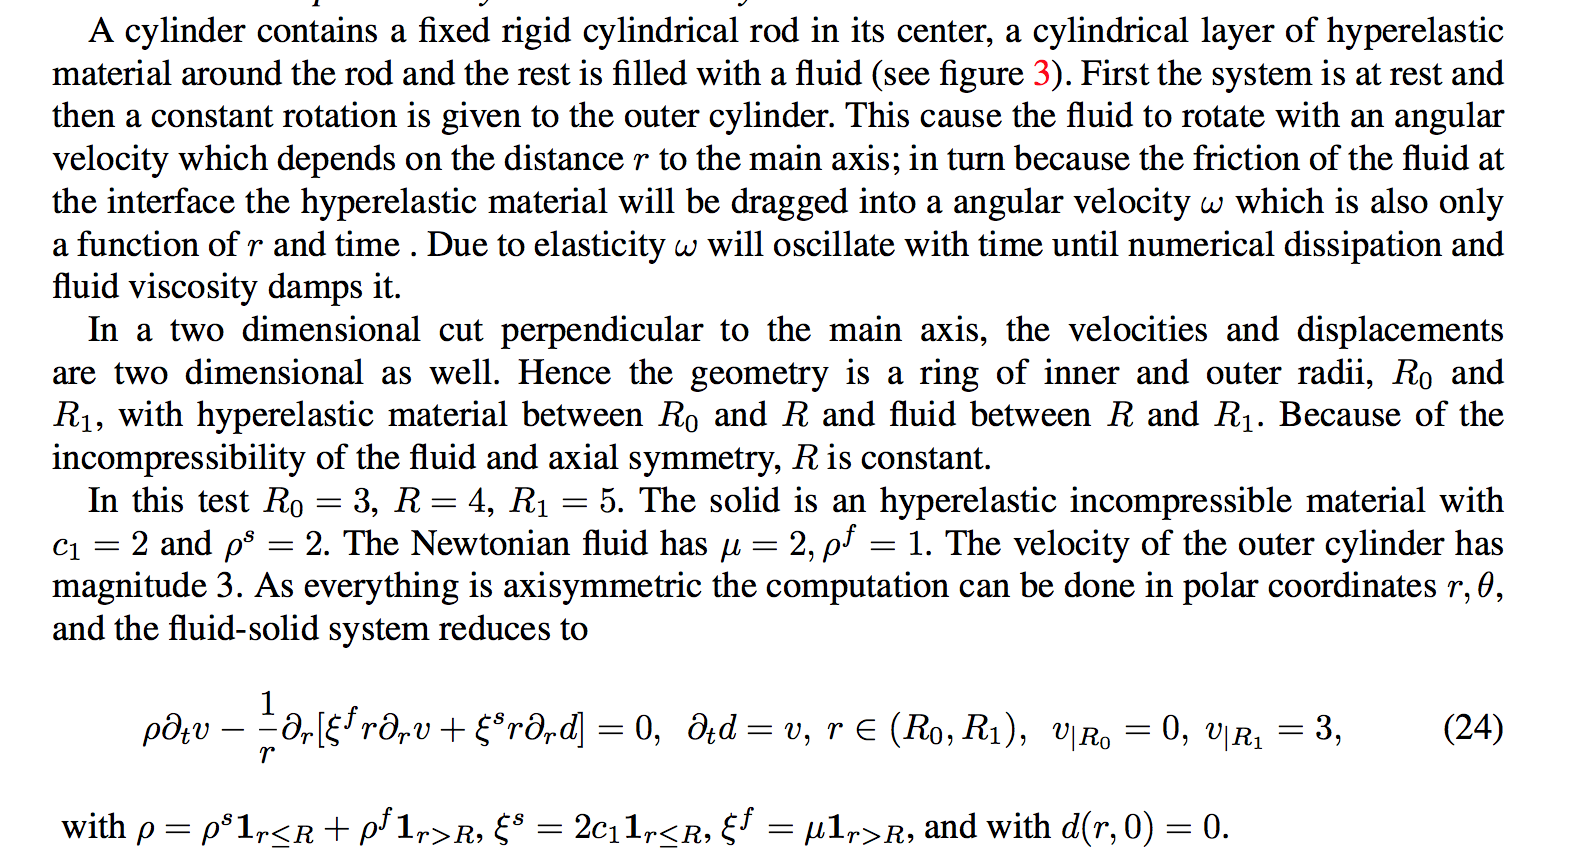
\includegraphics[width=14cm]{text.png}$$
\end{frame}
%
\begin{frame}[fragile] \manualFrameTitle{Example}
\small\bFF
@load "pipe"
@real R0=1,R1=2,R2=3,rhof=1,rhos=2,nu=1,kappa=5,v=3,T=0.8,dt=0.025;
/// semi-analytic solution by solving a 1d problem //
@mesh Th=square(100,5,[R0+(R2-R0)*x,0.1*y]);
@fespace Wh(Th,P1,periodic=[[1,x],[3,x]]);
@fespace W0(Th,P0);
Wh d=0,w,wh,wold=0;
W0 nnu=nu*(x>R1)+2*kappa*dt*(x<=R1), Rho=rhof*(x>R1)+rhos*(x<=R1);
@problem AA(w,wh) = int2d(Th)(Rho*x*w*wh/dt+x*nnu/2*dx(w)*dx(wh) )
			+ int2d(Th)(-Rho*x*wold*wh/dt +x*nnu/2*dx(wold)*dx(wh)
			+ 2*kappa*(x<=R1)*(x*dx(d)*dx(wh) ))
			+on(2,w=-v)+on(4,w=0);// this is the one-d axisymmetric problem
@pstream  pgnuplot("gnuplot" );  ////// prepare gnuplot ////
@int J=40;  @real dr = (R2-R0)/(J-1);
@for(int i=0;i<T/dt;i++){ 
   	AA; d=d+(w+wold)*dt; wold=w; 
   	@ofstream f("aux.gp");
   	@for(int j=0;j<J;j++) f << j*dr <<"   " << w(R0+j*dr,0.05) << endl;
   	pgnuplot << "plot 'aux.gp' u 1:2 w l "<< endl; 
   	@sleep(1); @flush(pgnuplot); 
}
\eFF
\end{frame}
%
\end{document}
\newslide{Summary} 
\begin{itemize}
\item Except \texttt{COMSOL} software to solve PDE are application oriented, like \texttt{NASTRAN,PamCrash,Abaqus,Fluent,OpenFOAM} etc.
\item \texttt{FreeFem++} is a software born in 2000 to solve numerically partial differential 
 equations (PDE)  in \Blue{$\mathrm{I\!R}^{2}$)}  and in \Red{$\mathrm{I\!R}^{3}$)} with finite elements methods. 
 
\item  It has its own language, as close to the mathematics as possible:  
  the \texttt{FreeFem++ script} which overwrites C++.  
  
\item  All PDEs are specified in variational form.  
 
\item  At the root  \texttt{FreeFem++} solves linear steady state problem and convection problems.
 
\item For time depend, nonlinear and coupled problem the user must specify the algorithm.
 
\item It can do mesh adaptation , compute error indicator, etc ...
\end{itemize}

\medskip
\Blue{  FreeFem++ is a freeware and this run on Mac, Unix and Window architecture, in parallel with MPI}.

\bigskip \vfill

%The next FreeFem workshop : Jussieu, Paris 5,6,7  December. 

\end{frame}

\subsection{The main characteristics} 
\newslide{The main characteristics \hfill \DarkGreen{(2D)}\Red{(3D)} }
{\begin{itemize}
\item Wide range of finite elements: {\small continuous P1,P2  elements, discontinuous P0, P1,  RT0,RT1,BDM1, elements ,Discontinuous-Galerkin, ...}

\item  \Blue{Automatic interpolation}  of data from a mesh to an other one, so a finite element 
function is view as a function of $(x,y\Red{,z})$ or as an array on the degree of Freedom.

\item \DarkGreen{Complex or real} functions with access  to  vectors and the
matrices.

\item {LU, Cholesky, Crout, CG, GMRES, UMFPack, { SuperLU, MUMPS, HIPS , SUPERLU\_DIST,
PASTIX.} ... } sparse linear solver; \Blue{eigenvalue} and  eigenvector computation with ARPACK.
%
\item Optimization Algorithms: GMRES, IPOPT, MEWUOA, CMAES etc.
\item \Blue{Automatic mesh generator}, based on Delaunay-Voronoi. (2d,\Red{3d} (tetgen) )
\item \Blue{Mesh adaptation based on automatic metric}, possibly anisotropic (only in 2d).
\item Link with other soft:  paraview, gmsh , vtk,   medit, gnuplot
\item Dynamic linking to add plugin. Full MPI interface
\item Online graphics with \Red{OpenGL/GLUT/VTK}, C++ like syntax.
\item An integrated development environment \Blue{ FreeFem++-cs (ann.jussieu.fr/lehyaric/ffcs)}

\end{itemize}}
\end{frame}

\begin{frame}\manualFrameTitle{Freefem++-CS integrated environment}
\includegraphics[height=10cm]{A_figs/freefemcs.png}
\end{frame}

\section{Basics}
\begin{frame}[fragile] \manualFrameTitle{Element of syntax 1/2}
\small\bFF
x,y,z , label, N.x, N.y, N.z, //  some reserved variables 
@int i = 0;  //  an integer
@real a=2.5; // a reel 
@bool b=(a<3.);
@real[@int]  array(10) ; // a real array of 10 value
@mesh Th;// a 2d mesh 
@fespace Vh(Th,P2); //Def. of  2d finite element space;
                 Vh u=x;  // a finite element function or array
@fespace V3h(Th,[P2,P2,P1]); V3h u;
                                      u(.5,.6,.7); u[];
Vh3<@complex> uc = x+ \textDarkGreen 1i\textBlack *y; // complex valued FE 
V3h [u1,u2,p]=[x,y,z];//a vectorial finite element 
@macro div(u,v) (dx(u)+dy(v))//EOM a macro 
@varf a([u1,u2,p],[v1,v2,q])=
            @int2d(Th)(  Grad(u1)'*Grad(v1) +Grad(u2)'*Grad(v2)
                 -div(u1,u2)*q -div(v1,v2)*p) +@on(1,2)(u1=g1,u2=g2);          
@matrix A=a(V3h,V3h,solver=UMFPACK);   
@real[int] b=a(0,V3h); 
u2[] =A^-1*b; // or you can put also u1[]=  or p[].
\eFF
\end{frame}
\begin{frame}[fragile] \manualFrameTitle{Element of syntax 2/2}
{\small\bFF
   @func Heaveside=(x>0);  // a formal line function 
   @func real g(int i, real a) { .....; return i+a;} 
   A = A + A'; A = A'*A ; A = [ [ A,0],[0,A'] ];
  @int[@int] I(15),J(15); // two array for renumbering
  @matrix B;
  B = A;   B=A(I,J); //  B(i,j) = A(I(i),J(j))       
  B=A(I^-1,J^-1);  // B(I(i),J(j))= A(i,j)        
  B.resize(10,20); //  resize the sparse matrix 
   @int[@int] I(1),J(1); @real[int] C(1);
  [I,J,C]=A; // get of the sparse term of the matrix A 
  A=[I,J,C]; // set a new matrix
  @matrix D=[diagofA] ; // set a diagonal matrix D 
  @real[int] a=2:12; //set  a[i]=i+2; i=0 to 10. 
  @complex a=1,b=2,c=3i;
  @func va=[ a,b,c];  // is a formal array in  [ ] 
  a =[ 1,2,3i]'*va ; cout << a << endl; // hermien product
  @matrix<complex>  A=va*[ 1,2,3i]'; cout << A << endl;
  a =[ 1,2,3i]'*va*2.;    a =(va+[ 1,2,3i])'*va*2.; 
  va./va; va*/va; // term to term /  and term to term *  
\eFF}
\end{frame}

\section{Academic Examples}
\subsection{Weak form}
\newslide{Laplace equation, weak form }

Let a domain $\Omega$ with a partition 
of $\partial\Omega$ in  $\Gamma_{2},  \Gamma_{e}$.

Find $u$ a solution in   such that:
\Blue{\begin{equation} 
- \Delta u = f \,\,  \mbox{in } \Omega , \quad  u=g \,  \mbox{ on }\, \Gamma_{2} , \quad \dn{u}=h\,  
\mbox{ on }\, \Gamma_{e}
\end{equation}}

Denote  $V_g = \{ v \in H^1(\Omega) / v_{|\Gamma_{2}} = g\} $ .

The Basic variationnal formulation with is: 
find $u \in V_{g}(\Omega)$  ,  such that 
\Blue{\begin{equation} 
\int_{\Omega }\nabla u.\nabla v  = \int_{\Omega} f v  \DarkGreen{+ \int_{\Gamma} h v}, 
\quad \forall v \in  V_{0}(\Omega)  
\end{equation}} \Magentab{The finite element method is just:  replace $ V_g$ with a finite element space, and the \texttt{FreeFem++} code: }

\end{frame}
\subsection{Poisson Equation}
\begin{frame}[fragile]
\manualFrameTitle{Poisson equation in a fish with FreeFem++}

The finite element method is just:  replace $ V_g$ with a finite element space, and the \texttt{FreeFem++} code: 

{\small\bFF
@mesh3 Th("fish-3d.msh");// read a mesh 3d
@fespace Vh(Th,@P1);   //  define the P1 EF space        

 Vh u,v;//set test and unknown function in Vh. 
@macro Grad(u) [dx(u),dy(u),dz(u)] //EOM Grad def
@func f=1;
@solve laplace(u,v,solver=CG) =
   @int3d(Th)(  Grad(u)'*Grad(v)   )   
   - @int3d(Th) ( f*v)
   + @on(2,u=2);   //  int on $\gamma_2$
@plot(u,fill=1,wait=1,value=0,wait=1);  


\eFF}


\Run{fish}\qquad
\Run{fish3d}
%\qquad\Run{EqPoisson}

\end{frame}

\section{Tools}
\subsection{Remarks on weak form and boundary conditions}


\section{Mesh generation}

%\subsection{Mesh generation}
\begin{frame}[fragile]
\manualFrameTitle{Build Mesh 2d}

a L shape domain $]0,1[^2 \backslash  [\frac{1}{2},1[^2$

{ \bFF
@border a(t=0,1.0){x=t;   y=0;  label=1;};            
@border b(t=0,0.5){x=1;   y=t;  label=1;};
@border c(t=0,0.5){x=1-t; y=0.5;label=1;};            
@border d(t=0.5,1){x=0.5; y=t;  label=1;};
@border e(t=0.5,1){x=1-t; y=1;  label=1;};            
@border f(t=0.0,1){x=0;   y=1-t;label=1;}; 
@plot(a(6)+b(4)+c(4)+d(4)+e(4)+f(6),wait=1); // to see 
@mesh Th2 =  @buildmesh (a(6)+b(4)+c(4)+d(4)+e(4)+f(6)); 
\eFF}

\end{frame}

\begin{frame}[fragile]\manualFrameTitle{boundary  mesh of a Sphere}
{\small \bFF
@load "tetgen"
@mesh Th=square(10,20,[x*pi-pi/2,2*y*pi]);  //  $]\frac{-pi}{2},\frac{-pi}{2}[\times]0,2\pi[ $
@func f1 =cos(x)*cos(y); @func f2 =cos(x)*sin(y); @func f3 = sin(x);
//  the  partiel derivative of the parametrization DF
@func f1x=sin(x)*cos(y);    @func f1y=-cos(x)*sin(y);
@func f2x=-sin(x)*sin(y);   @func f2y=cos(x)*cos(y);
@func f3x=cos(x);           @func f3y=0;
// $  M = DF^t DF $
@func m11=f1x^2+f2x^2+f3x^2;  @func m21=f1x*f1y+f2x*f2y+f3x*f3y;
@func m22=f1y^2+f2y^2+f3y^2;
@func perio=[[4,y],[2,y],[1,x],[3,x]];  
@real hh=0.1/R; @real vv= 1/square(hh);
Th=adaptmesh(Th,m11*vv,m21*vv,m22*vv,IsMetric=1,periodic=perio);  
int[int] ref=[0,L]; // the label of the Sphere to L  ( 0 -> L) 
@mesh3  ThS= movemesh23(Th,transfo=[f1*R,f2*R,f3*R],orientation=1,
   label=ref);
\eFF}
\Run{Sphere} \Run{sphere6} 
\end{frame}

\subsection{Mesh tools}
\newslide{Mesh tools}
\begin{itemize}
\item \texttt{change}  to change label and region numbering in 2d and 3d.
\item \texttt{movemesh} \texttt{checkmovemesh} \texttt{movemesh23} \texttt{movemesh3}
\item \texttt{triangulate} (2d) , \texttt{tetgconvexhull} (3d)  build mesh mesh for a set of point 
\item \texttt{emptymesh} (2d) built a empty mesh for Lagrange multiplier
\item \texttt{freeyams}  to optimize surface mesh 
\item \texttt{mmg3d} to optimize volume mesh with constant surface mesh 
\item \texttt{mshmet} to compute metric
\item \texttt{isoline} to extract isoline (2d)
\item \texttt{trunc} to remove peace of mesh and split all element (2d,3d)
\item \texttt{splitmesh} to split  2d mesh  in no regular way. 
\end{itemize}

\end{frame}
\newslide{A corner singularity \hglue 1.5cm  {\normalsize adaptation with metric}}
    
The domain is an L-shaped polygon $\Blue{\Omega}= ]0,1[^2 \backslash 
[\frac{1}{2},1] ^2$ and the PDE is
$$
\hbox{ Find $u\in H^1_0( \Blue{\Omega})$ such that ~}
-\Delta u = 1~\hbox{in~} \Blue{\Omega},
$$ 
The solution has a singularity at the reentrant angle and we wish to 
capture it
numerically.

\medskip

\LINE{\hss\includegraphics[height=3.5cm]{L-a-Mesh01} \hss 
\includegraphics[height=3.5cm]{L-a-Mesh07}\hss}
\LINE{ \hss example of Mesh adaptation \hss }
\end{frame}

\begin{frame}[fragile]{ FreeFem++ corner singularity program}
\small\bFF
@int[@int] lab=[1,1,1,1];
@mesh Th = @square(6,6,label=lab);
Th=@trunc(Th,x<0.5 | y<0.5, label=1);

@fespace Vh(Th,P1);         Vh u,v;         real error=0.1;
@problem Probem1(u,v,solver=CG,eps=1.0e-6) =
       @int2d(Th)(  dx(u)*dx(v) + dy(u)*dy(v))  
     - @int2d(Th)( v) + @on(1,u=0);
@for (@int i=0;i< 7;i++)
{  Probem1;                         // solving the pde  
   Th=adaptmesh(Th,u,err=error,nbvx=100000);   
   //  the adaptation with Hessian of $u$
   plot(Th,u,wait=1,fill=1);           u=u;      
   error = error/ (1000.^(1./7.)) ;   } ;
\eFF

\bigskip
\Run{CornerLap}
\end{frame}



\subsection{3d Poisson equation with mesh adaptation}
\begin{frame}[fragile]
\manualFrameTitle{Poisson equation with 3d mesh adaptation}% on $]0,1[^3\setminus[1/2,1[^3 $}
\tiny\bFF
@load "msh3" load "tetgen" load "mshmet" load "medit"
@int nn  = 6;
@int[@int] l1111=[1,1,1,1],l01=[0,1],l11=[1,1];//   label numbering 
@mesh3 Th3=@buildlayers(square(nn,nn,region=0,label=l1111),
      nn,  zbound=[0,1], labelmid=l11,labelup = l01,labeldown = l01);
Th3=@trunc(Th3,(x<0.5)|(y < 0.5)|(z < 0.5) ,label=1);// remove  $]0.5,1[^3$
\eFF\scriptsize\bFF
@fespace Vh(Th3,P1);      Vh u,v;//FE.  space definition
@macro @Grad(u) [dx(u),dy(u),dz(u)] // EOM
@problem @Poisson(u,v,solver=CG) =
  @int3d(Th3)( @Grad(u)'*@Grad(v) )  -@int3d(Th3)( 1*v ) + @on(1,u=0);
  
@real errm=1e-2;// level of error 
@for(@int ii=0; ii<5; ii++)
{
  Poisson;        Vh h;      
  h[]=@mshmet(Th3,u,normalization=1,aniso=0,nbregul=1,hmin=1e-3,
             hmax=0.3,err=errm);
  errm*= 0.8;// change the level of error
  Th3=@tetgreconstruction(Th3,switch="raAQ"
        ,sizeofvolume=h*h*h/6.);
  @medit("U-adap-iso-"+ii,Th3,u,wait=1);
}
\eFF
\Run{Laplace-Adapt-3d}\hfill
\end{frame}
\section{Linear PDE}


\subsection{Linear elasticty equation}
%\newslide{Linear elasticty equation, weak form }


\begin{frame}[fragile]
\manualFrameTitle{Linear Lame equation, weak form }

Let a domain $\Omega\subset \mathbb{R}^d $ with a partition 
of $\partial\Omega$ in  $\Gamma_{d},  \Gamma_{n}$.

Find the displacement $\bm{u}$ field such that:
\Blue{\begin{equation} 
- \nabla.\sigma(\bm{u}) = \bm{f} \,\,  \mbox{in } \Omega , \quad  \bf{u}=\bm{0} \,  \mbox{ on }\, \Gamma_{d} , \quad \sigma(\bm{u}).\bm{n}=0\,  
\mbox{ on }\, \Gamma_{n}
\end{equation}}
Where $ \varepsilon(\bm{u}) = \frac12(\nabla \bm{u} + {}^t\nabla \bm{u})$ and $ \sigma(\bm{u}) = \bm{A} \varepsilon(\bm{u})$ with 
$\bm{A} $ the linear  positif operator on symmetric $d\times d$ matrix corresponding to the material propriety. 
Denote  $V_{\bm{g}}= \{ \bm{v} \in H^1(\Omega)^d / \bm{v}_{|\Gamma_{d}} = \bm{g}\} $ .

The Basic displacement variational formulation is: 
find $\bm{u} \in V_{0}(\Omega)$,  such that: 
\Blue{\begin{equation} 
\int_{\Omega }  \varepsilon(\bm{v}) :\bm{A}\varepsilon(\bm{u})= \int_{\Omega} \bm{v}.\bm{f}  \DarkGreen{+ \int_{\Gamma} ((\bm{A}\varepsilon(\bm{u})).n). v}, 
\quad \forall \bm{v} \in  V_{0}(\Omega)  
\end{equation}} 
\end{frame}

\begin{frame}[fragile]
\manualFrameTitle{Linear elasticty equation, in FreeFem++}
The finite element method is just:  replace $ V_g$ with a finite element space, and the \texttt{FreeFem++} code: 
\small 
\bFF
@load "medit"   @include "cube.idp"
@int[@int]  Nxyz=[20,5,5];
@real [@int,@int]  Bxyz=[[0.,5.],[0.,1.],[0.,1.]];
@int [@int,@int]  Lxyz=[[1,2],[2,2],[2,2]];
@mesh3 Th=Cube(Nxyz,Bxyz,Lxyz);
// Alu ...
@real rhoAlu = 2600, alu11=  1.11e11 , alu12 = 0.61e11 ;
@real alu44= (alu11-alu12)*0.5;
@func Aalu = [  [alu11, alu12,alu12,   0.   ,0.   ,0.  ],
               [alu12, alu11,alu12,   0.   ,0.   ,0.   ],
               [alu12, alu12,alu11,   0.   ,0.   ,0.   ],
               [0. ,   0. ,   0. ,    alu44,0.   ,0.   ],
               [0. ,   0. ,   0. ,    0.   ,alu44,0.   ],
               [0. ,   0. ,   0. ,    0.   ,0.   ,alu44]   ];
@real gravity = -9.81;
\eFF
\end{frame}


\begin{frame}[fragile]
\manualFrameTitle{Linear elasticity equation, in FreeFem++}


\scriptsize\bFF
@fespace Vh(Th,[P1,P1,P1]);
Vh [u1,u2,u3], [v1,v2,v3];
@macro Strain(u1,u2,u3) 
  [ dx(u1), dy(u2),dz(u3), 
  (dz(u2) +dy(u3)), (dz(u1)+dx(u3)),
   (dy(u1)+dx(u2)) ] // EOM
@solve Lame([u1,u2,u3],[v1,v2,v3])=
  @int3d(Th)(  
      Strain(v1,v2,v3)'*(Aalu*Strain(u1,u2,u3))  )
- @int3d(Th) ( rhoAlu*gravity*v3)  
      + @on(1,u1=0,u2=0,u3=0) ;
           
@real coef= 0.1/u1[].linfty;  @int[@int] ref2=[1,0,2,0];
@mesh3 Thm=movemesh3(Th,
     transfo=[x+u1*coef,y+u2*coef,z+u3*coef],
     label=ref2);
@plot(Th,Thm, wait=1,cmm="coef  amplification = "+coef );
@medit("Th-Thm",Th,Thm);
\eFF
\end{frame}


%\section{Lame equation in 3d}
\begin{frame}[fragile]
\manualFrameTitle{Lame equation / figure }
\HLINE{\includegraphics[width=6cm]{beam-3d.jpg}\hss
\includegraphics[width=6cm]{beam-ev.jpg}}

\small \Run{beam-3d}\hfill\Run{beam-EV-3d}\hfill
\Run{beam-3d-Adapt}
%\Run{fish}
%\Run{Laplace3d}
%\Run{EqPoisson}

\end{frame}

\subsection{Stokes equation}
\begin{frame}[fragile]
\manualFrameTitle{Stokes  equation}

The Stokes equation is find a velocity field $\bm{u}=(u_1,..,u_d)$ and the pressure $p$ 
on domain $\Omega$ of $\mathbb{R}^d$, such that 
\Blue{\begin{eqnarray*}
     -\Delta \bm{u} + \nabla p &=0 & \quad  \mbox{in} \quad \Omega 
    \cr
    \nabla\cdot  \bm{u} &=0& \quad  \mbox{in} \quad \Omega
    \cr
    \bm{u}  & = \bm{u}_\Gamma &  \quad  \mbox{on} \quad \Gamma
\end{eqnarray*}}

where $\bm{u}_\Gamma$ is a given velocity on boundary $\Gamma$.


The classical variational formulation is: Find $\bm{u} \in H^1(\Omega)^d $ with $  \bm{u}_{\vert\Gamma} = u_\Gamma$, and
$p\in L^2(\Omega)/\mathbb{R}$ such that
$$
\forall \bm{v} \in H^1_0(\Omega)^d,\ \forall q \in L^2(\Omega)/\mathbb{R},
\qquad   \Blue{ \int_\Omega \nabla \bm{u}: \nabla \bm{v} - p \nabla. v - q  \nabla. u = 0}
$$

or now find $p\in L^2(\Omega)$ such than (with $\varepsilon=10^{-10}$)
$$
\forall \bm{v} \in H^1_0(\Omega)^d,\ \forall q \in L^2(\Omega)  ,  \Blue{   \int_\Omega \nabla \bm{u}: \nabla \bm{v} - p \nabla. v - q  \nabla. u + \Rose{\varepsilon p q} = 0 }
$$

\end{frame}


\begin{frame}[fragile]
\manualFrameTitle{Stokes  equation in FreeFem++}
\bFF
\textRed ...  build mesh .... Th (3d) T2d ( 2d)
@fespace VVh(Th,[P2,P2,P2,P1]);// Taylor Hood FE.
@macro Grad(u) [dx(u),dy(u),dz(u)]// EOM\hfill
@macro div(u1,u2,u3) (dx(u1)+dy(u2)+dz(u3)) //EOM\hfill
VVh [u1,u2,u3,p],[v1,v2,v3,q] ;
solve vStokes([u1,u2,u3,p],[v1,v2,v3,q]) = 
  @int3d(Th)( 
          Grad(u1)'*Grad(v1) 
       +  Grad(u2)'*Grad(v2) 
       +  Grad(u3)'*Grad(v3)
     - div(u1,u2,u3)*q - div(v1,v2,v3)*p 
     - 1e-10*q*p ) 
 + @on(1,u1=0,u2=0,u3=0)   +  @on(2,u1=1,u2=0,u3=0);

\eFF
\Run{Stokes3d}
\end{frame}


\section{Numerics Tools}

\subsection{Eigenvalue}
\begin{frame}[fragile]
\manualFrameTitle{Eigenvalue/ Eigenvector example}

 The problem, Find the first $\lambda, u_\lambda$ such that:
 \Blue{$$ a( u_\lambda,v) = \int_{\Omega}  \nabla u_\lambda \nabla v = \lambda \int_{\Omega} u_\lambda   v = \lambda  b(u_\lambda,v) $$}

the boundary condition is make with exact penalization:
     we put $1e30=tgv$  on the diagonal term of the lock degree of freedom.
So take Dirichlet boundary condition only  with  $a$ variational form
and not on  $b$ variational form , because we compute eigenvalue of 
 $$ w=A^{-1} B v $$
Otherwise we get spurious mode. 

Arpack interface: 
\bFF
@int k=EigenValue(A,B,sym=true,value=ev,vector=eV);
\eFF
\end{frame}
\subsection{Eigenvalue/ Eigenvector}
\begin{frame}[fragile]
\manualFrameTitle{Eigenvalue/ Eigenvector example code}
\small
\bFF
... 
@fespace Vh(Th,P1);
@macro Grad(u) [dx(u),dy(u),dz(u)] // EOM
@varf  a(u1,u2)= int3d(Th)(  Grad(u1)'*Grad(u2) +  on(1,u1=0) ;                    
@varf b([u1],[u2]) = int3d(Th)(  u1*u2 ) ; // no BC
@matrix A= a(Vh,Vh,solver=UMFPACK),
        B= b(Vh,Vh,solver=CG,eps=1e-20);
 
@int nev=40;// number of computed eigenvalue close to 0
@real[@int] ev(nev); // to store nev eigenvalue
@Vh[int] eV(nev);   // to store nev eigenvector
@int k=EigenValue(A,B,sym=true,value=ev,vector=eV);
k=min(k,nev); 
@for (@int i=0;i<k;i++)
   plot(eV[i],cmm="ev  "+i+" v =" + ev[i],wait=1,value=1);
\eFF
\edpRun{Lap3dEigenValue}\hglue 2cm  \edpRun{LapEigenValue}
\end{frame}


%\subsection{Optimization Tools}

%\subsection{Variational  Inequation}

\subsection{Optimization: Ipopt interface}

\begin{frame}[fragile]
\manualFrameTitle{Ipopt optimizer}

The IPOPT optimizer in a FreeFem++ script is done with the {\tt IPOPT} function included in the {\tt ff-Ipopt} dynamic library. IPOPT is designed to solve constrained minimization problem in the form :

{\color{blue} \begin{equation*}\label{ipoptproblem}
 \begin{array} {r l}
     \mathrm{find}& x_{0} = \underset{x\in\R^{n}}{\operatorname{argmin}} f(x) \\
     \mathrm{s.t.}&\left\lbrace \begin{array}{l r}  \forall i\leq n,\ x_{i}^{\mathrm{lb}}\leq x_{i}\leq x_{i}^{\mathrm{ub}} & \mathrm{\  (simple\ bounds)} \\
       \forall i\leq m,\ c_{i}^{\mathrm{lb}}\leq c_{i}(x)\leq c_{i}^{\mathrm{ub}} & \mathrm{(constraints\ functions)}
 \end{array}\right. \\
 
 \end{array}
 \end{equation*}}
Where $\mathrm{ub}$ and $\mathrm{lb}$ stand for "upper bound" and "lower bound". If for some $i, 1\leq i\leq m$ we have $c_{i}^{\mathrm{lb}} = c_{i}^{\mathrm{ub}}$, it means that $c_{i}$ is an equality constraint, and an inequality one if $c_{i}^{\mathrm{lb}} < c_{i}^{\mathrm{ub}}$.

{\scriptsize
\bFF
  @func @real J(@real[@int] &X) {...} //Fitness Function,
  @func @real[@int] gradJ(@real[@int] &X) {...} //Gradient 
  @func @real[int] C(@real[@int] &X) {...} //Constraints
  @func @matrix jacC(@real[@int] &X) {...} //Constraints jacobian
  @matrix jacCBuffer; //just declare, no need to define yet
  @func @matrix jacC(@real[@int] &X) 
    {...  @return jacCBuffer; }  //fill jacCBuffer 
\eFF}

\end{frame}

\begin{frame}[fragile]
\manualFrameTitle{Stochastic  Optimizer}


This algorithm works with a normal multivariate distribution in the parameters
space and try to adapt its covariance matrix using the information provides by
the successive function evaluations. Syntaxe: \texttt{cmaes(J,u[],..)} ( )

 

From \url{http://www.lri.fr/~hansen/javadoc/fr/inria/optimization/cmaes/package-summary.html}

%\scriptsize
\bFF
@load  "mpi-cmaes" 

@real mini = @cmaesMPI(J,start,stopMaxFunEval=10000*(al+1),
                stopTolX=1.e-4/(10*(al+1)),
                initialStdDev=(0.025/(pow(100.,al))));
SSPToFEF(best1[],best2[],start);

\eFF
\Run{cmaes-VarIneq}  %\Run{cmaes-oven}

\end{frame}


\section{Incompressible Navier-Stokes equations}
\begin{frame}{incompressible Navier-Stokes  equation with characteristics methods}
\Blue{$$
    {\p {u}\over\p t} +(u\cdot\nabla) u-\nu \Delta u+\nabla p=0,~~~ \nabla\cdot u=0
$$}
with the same boundary conditions and with initial conditions $u=0$.

This is implemented by using the interpolation  operator for the term
${\p u\over\p t} +(u\cdot\nabla) u$, giving a discretization in time
\Blue{\index{Navier-Stokes}
\begin{equation}
    \label{eq Navier Stokes carac}
\begin{array}{cl}
\frac{1}{\tau } (u^{n+1}-u^n\circ X^n) -\nu\Delta u^{n+1} + \nabla p^{n+1} &=0,\\
 \nabla\cdot u^{n+1} &= 0
 \end{array}
\end{equation}
}
The term $ X^n(x)\approx  x-\tau u^n(x) $ will be
computed by the interpolation operator or convect operator. 

Or better we use an  order 2 schema, BDF1 
\Blue{$$
  {\p {u}\over\p t} + (u\cdot\nabla) u \approx   \frac{(3 u^{n+1} -4  u^n\circ X_1^n + u^{n-1}\circ X_2^n) }{2 \tau }
$$}
with $u^{*}= 2 u^n - u^{n-1}  $, and $X_1^n(x)\approx  x-\tau u^{*}(x), X_2^n(x)\approx  x-2\tau u^{*}(x) $

\Run{NSCaraCyl-100-mpi}
\end{frame}
\subsection{Boussinesq equation}
\begin{frame}{Natural Convection}
\small 

 The coupling of natural convection modeled by the Boussinesq approximation and liquid to solid phase change in $\Omega = ]0,1[^2 $, 
 No slip condition for the fluid are applied at the boundary and  adiabatic condition on upper and lower boundary and given temperature $\theta_r$ (resp $\theta_l$) at  the right  and left boundaries. 

The model is: find the field : the velocity $\bm{u}=(u_1,u_2)$, the pressure $p$  and temperature $\theta$ : 
\Blue{\begin{equation}
\left\{\begin{array}{rll}
%\bm{u} & \hbox{ given } & \mbox{ in }\Omega \\
 \p_t\bm{u} + (\bm{u}.\nabla) \bm{u}  + \nabla. \mu\nabla   \bm{u} + \nabla p &= - C_T (\theta-\theta_0)  \bm{e}_2 &\mbox{ in }\Omega \\
  \nabla.\bm{u} & = 0 &  \mbox{ in }\Omega \\
 %
 \p_t \theta + (\bm{u}.\nabla) \theta + \nabla. k_T \nabla \theta & = 0 & \mbox{ in }\Omega  \\
\end{array}  \right.\label{orange} 
\end{equation}}
Where $C_T (\theta-\theta_0)  \bm{e}_2 $ correspond to the Archimedes forces due  to the  affine dependence of density with the temperature and where $\theta_0$ is temperature
of the reference density. 


\bigskip
\Run{boussinesq2d} \hfill \Run{boussinesq3d} \hfill \Run{boussinesq3d-mpi}
\end{frame}


\section{Phase change with Natural Convection}

\begin{frame}\manualFrameTitle{Phase change with Natural Convection}
\small 
The starting point of the problem  is Brainstorming session (part I) of  the third  {FreeFem++} days in december 2011, this is  almost the Orange Problem is describe in web  page \url{http://www.ljll.math.upmc.fr/~hecht/ftp/ff++days/2011/Orange-problem.pdf}.

 The coupling of natural convection modeled by the Boussinesq approximation and liquid to solid phase change in $\Omega = ]0,1[^2 $, 
 No slip condition for the fluid are applied at the boundary and  adiabatic condition on upper and lower boundary and given temperature $\theta_r$ (resp $\theta_l$) at  the right  and left boundaries. 

The model is: find the field : the velocity $\bm{u}=(u_1,u_2)$, the pressure $p$  and temperature $\theta$ : 
\Blue{\begin{equation}
\left\{\begin{array}{rll}
\bm{u} & \hbox{ given } & \mbox{ in }\Omega_s \\
 \p_t\bm{u} + (\bm{u} \nabla) \bm{u}  + \nabla. \mu\nabla   \bm{u} + \nabla p &= - c_T \bm{e}_2 &\mbox{ in }\Omega_f \\
  \nabla.\bm{u} & = 0 &  \mbox{ in }\Omega_f \\
 %
 \p_t \theta + (\bm{u} \nabla) \theta + \nabla. k_T \nabla \theta & = \p_t S(T) & \mbox{ in }\Omega  \\
\end{array}  \right.\label{orange} 
\end{equation}}
Where $\Omega_f$ is the fluid domain  and the solid domain is $\Omega_s=\Omega\setminus \Omega_f$.  
\end{frame}

\begin{frame}\manualFrameTitle{Phase change with Natural Convection}

The enthalpy of the 
change of phase is given by the function $S$; $\mu$ is the relative viscosity, $k_T$  the thermal diffusivity.

In $\Omega_f = \{ x \in \Omega ; \theta > \theta_f \}  $, with $ \theta_m$  the melting  temperature the solid has melt. 


We modeled, the solid phase as a fluid   with huge viscosity, so : 
$$ \mu = \left\{\begin{array}{ccc} \theta < \theta_f  &\sim& 10^6  \\
 \theta \ge  \theta_m &\sim& \frac1{\mathrm{Re}} \end{array}\right., $$
% This removes movement in the solid phase, and here $\mathrm{Re}$ is the Reynolds number of the liquid phase.   
 The Stefan  enthalpy $S_c$ with defined by
$ S_c(\theta) = H(\theta)/S_{th}$ where $S_{the}$ is the stefan number, 
and  $H$ is the Heaviside function
with use the following smooth the enthalpy:
$$ S(\theta) = \frac{\tanh(50 (\theta-\theta_m) ))}{2 S_{te}}.$$
\end{frame}

\begin{frame}\manualFrameTitle{The Physical Device}
\includegraphics[width=\hsize]{plots/Fig-orange.pdf}
\end{frame}

\begin{frame}[fragile]\manualFrameTitle{the Algorithm}

We apply a fixed point algorithm for the phase change part (the domain $\Omega_f$ is fixed at each iteration) and a full no-linear  Euler implicit 
scheme with a fixed  domain for the rest.
We use a Newton method to solve the non-linearity. 

\begin{itemize}
\item if we don't make mesh adaptation, the Newton method do not converge
\item if we use explicit  method   diverge too,
\item if we implicit the dependance in $\Omega_s$ the method also diverge.
\end{itemize}   
\Blue{  Implementation}
The finite element space to approximate  $u1,u2,p,\theta$ is defined by 
\begin{lstlisting}
 fespace Wh(Th,[P2,P2,P1,P1]);
\end{lstlisting}
We do mesh adaptation a each time step, with the following code:
\begin{lstlisting}
  Ph ph = S(T), pph=S(Tp);
  Th= adaptmesh(Th,T,Tp,ph,pph,[u1,u2],err=errh,
                hmax=hmax,hmin=hmax/100,ratio = 1.2);
\end{lstlisting}
This mean,  we adapt   all variables, the 2 melting phase a time $n+1$ and ${n}$  and smooth the metric with a ratio of $1.2$ to  account for the motion of the melting front.
\end{frame}

\begin{frame}[fragile]\manualFrameTitle{The Newton loop}

the fixed point are implemented as follows
\begin{lstlisting}
  real err=1e100,errp ;
   for(int kk=0;kk<2;++kk) // 2 step of fixe point on $\Omega_s$ 
   { nu = nuT; // recompute the viscosity in $\Omega_s,\Omega_f$ 
     for(int niter=0;niter<20; ++ niter) // newton loop 
      { BoussinesqNL; 
        err = u1w[].linfty;
        cout << niter << " err NL " << err <<endl; 
        u1[] -= u1w[];    
        if(err < tolNewton) break;  }// convergence ..
    }
\end{lstlisting}
%
\end{frame}
\begin{frame}[fragile]\manualFrameTitle{The linearized problem}\tiny
\vglue-0.5cm\begin{lstlisting}
problem BoussinesqNL([u1w,u2w,pw,Tw],[v1,v2,q,TT])
= int2d(Th) (
     [u1w,u2w,Tw]'*[v1,v2,TT]*cdt
     + UgradV(u1,u2,u1w,u2w,Tw)' * [v1,v2,TT]
     + UgradV(u1w,u2w,u1,u2,T)' * [v1,v2,TT]
     + ( Grad(u1w,u2w)'*Grad(v1,v2)) * nu 
     + ( Grad(u1,u2)'*Grad(v1,v2)) * dnu* Tw   
     + cmT*Tw*v2  + grad(Tw)'*grad(TT)*kT  
     - div(u1w,u2w)*q -div(v1,v2)*pw - eps*pw*q 
     + dS(T)*Tw*TT*cdt )
   - int2d(Th)(
     [u1,u2,T]'*[v1,v2,TT]*cdt
     + UgradV(u1,u2,u1,u2,T)' * [v1,v2,TT]
     + ( Grad(u1,u2)'*Grad(v1,v2)) * nu 
     + cmT*T*v2 - eps*p*q  +  grad(T)'*grad(TT)*kT  
     - div(u1,u2)*q -div(v1,v2)*p 
     +  S(T)*TT*cdt - [u1p,u2p,Tp]'*[v1,v2,TT]*cdt 
     -  S(Tp)*cdt*TT) 
 + on(1,2,3,4, u1w=0,u2w=0)+on(2,Tw=0)+on(4,Tw=0) ;
\end{lstlisting}
\end{frame}

\begin{frame}\manualFrameTitle{The parameters of the computation} 

  take  case 2 from 
  
  
  Shimin Wang, Amir Faghri, and Theodore~L. Bergman. {A comprehensive numerical model for melting with natural
  convection}. {\em International Journal of Heat and Mass Transfer}, January 2010.
 
 \bigskip   
$\theta_m=0$, 
$\mathrm{Re}=1$, $S_{te}=0.045$, $P_{r}= 56.2$, 
 $R_a =  3.27\ 10^5$ , $\theta_l = 1, \theta_r = -0.1$ 
 so in this case $ \mathrm{cmT}=c_T=-R_a/P_{r}$ , $\mathrm{kT} = k_T = 1/P_r$, $\mathrm{eps}=10^{-6}$,
 time step $\delta t = 10^{-1}$, $\mathrm{cdt}=1/\delta t$, at time $t=80$  and we get  a good agreement with 
 the article.   
 

 

   
 

\end{frame}

\begin{frame}\manualFrameTitle{Phase change with Natural Convection}

\bigskip
\includegraphics[width=5cm]{OT.jpg}\hfill
\includegraphics[width=5cm]{OU.jpg}

\Blue{So now, a real problem, get the physical parameter of the real experiment.}

\Run{Orange-Newton}
\end{frame}

\begin{frame}[fragile]\manualFrameTitle{Conclusion/Future}
\vfill 
Freefem++ v3.20 is  
\begin{itemize}
\item very good tool to solve non standard PDE in 2D/3D
\item to try new domain decomposition domain algorithm
\end{itemize}

\vfill 
The the future we try to do:
\begin{itemize}
\item Build more graphic with VTK, paraview , ... (in progress)
\item Add Finite volume facility for hyperbolic PDE (just begin C.F.  FreeVol Projet)
\item 3d anisotrope mesh adaptation
\item automate the parallel tool 
\end{itemize}

\vfill 
Thank for you attention. 
 \label{LastPage}
\end{frame}


\end{document}